\documentclass[10pt, twocolumn]{article}
\usepackage[a4paper, margin=0.5in, top=0.5in, bottom=0.5in]{geometry}
\usepackage{amsmath}
\usepackage{booktabs}
\usepackage{xcolor}
\usepackage{listings}
\usepackage{enumitem}
\usepackage[compact]{titlesec}
\usepackage{tikz}
\usetikzlibrary{shapes.geometric, arrows.meta, positioning, matrix, fit, calc, decorations.pathreplacing}

% --- These commands make all lists and headings more compact ---
\setlist{nosep, leftmargin=*, itemsep=0pt, topsep=2pt, partopsep=0pt}
\titlespacing*{\section}{0pt}{*1}{*1}
\titlespacing*{\subsection}{0pt}{*0.5}{*0.5}
\titlespacing*{\subsubsection}{0pt}{*0.5}{*0.5}
\setlength{\columnsep}{1cm}

\tikzstyle{arrow} = [thick,->,>=stealth]

% Define a style for code listings
\lstdefinestyle{mystyle}{
    commentstyle=\color{gray},
    keywordstyle=\color{blue},
    stringstyle=\color{purple},
    basicstyle=\ttfamily\scriptsize,
    breakatwhitespace=false,
    breaklines=true,
    keepspaces=true,
    numbers=none,
    showstringspaces=false,
}
\lstset{style=mystyle}

\pagestyle{empty} % Removes page numbers

\begin{document}

\section*{Machine-Level Programming I}

\subsection*{Intel Processor History \& Compilation}
\begin{itemize}
    \item \textbf{Intel x86:} Dominant CISC architecture, backward-compatible.
    \item \textbf{Milestones:} \textbf{8086} (16-bit), \textbf{386} (32-bit IA32), \textbf{Pentium 4E} (64-bit x86-64), \textbf{Core 2} (multi-core).
    \item \textbf{Compilation:} C Code $\xrightarrow{\text{Compiler (gcc -S)}}$ Assembly $\xrightarrow{\text{Assembler (as)}}$ Object Code $\xrightarrow{\text{Linker (ld)}}$ Executable.
\end{itemize}

\subsection*{Assembly Basics}
\begin{table}[h]
    \centering
    \caption{Key x86-64 Registers}
    \scriptsize
    \begin{tabular}{@{}lll@{}}
        \toprule
        Register & Role & Saved By \\
        \midrule
        \%rax & Return Value & Caller \\
        \%rdi, \%rsi, \%rdx, \%rcx & Arguments 1-4 & Caller \\
        \%r8, \%r9 & Arguments 5-6 & Caller \\
        \%r10, \%r11 & Temporaries & Caller \\
        \%rbx, \%r12-\%r15 & Temporaries & Callee \\
        \%rsp, \%rbp & Stack/Base Pointer & Callee \\
        \bottomrule
    \end{tabular}
\end{table}

\subsubsection*{Addressing Modes}
General Form: \textbf{\texttt{D(Rb, Ri, S) $\rightarrow$ Mem[Rb + S*Ri + D]}}
\begin{itemize}
    \item \textbf{D:} Displacement (constant)
    \item \textbf{Rb:} Base register
    \item \textbf{Ri:} Index register
    \item \textbf{S:} Scale factor (1, 2, 4, or 8)
\end{itemize}
\textbf{Examples:}
\begin{lstlisting}[language=c, basicstyle=\ttfamily\tiny]
// Immediate: Constant data
movq $0x4, %rax
// Register: Data in a register
movq %rax, %rdx
// Memory: Data at an address
movq (%rax), %rdx // Normal
movq 8(%rbp), %rdx // Displacement
\end{lstlisting}

\subsection*{Arithmetic \& Logical Operations}
\begin{table}[h]
    \centering
    \caption{Common Instructions (q=8, l=4, w=2, b=1)}
    \scriptsize
    \begin{tabular}{@{}ll@{}}
        \toprule
        Instruction & Description \\
        \midrule
        \texttt{leaq Src, Dst} & Load Effective Address (address calc) \\
        \texttt{addq Src, Dst} & Add: Dst = Dst + Src \\
        \texttt{subq Src, Dst} & Subtract: Dst = Dst - Src \\
        \texttt{imulq Src, Dst} & Multiply: Dst = Dst * Src \\
        \texttt{salq/shlq k, Dst} & Left Shift: Dst = Dst << k \\
        \texttt{sarq/shrq k, Dst} & Right Shift (Arith/Logical) \\
        \texttt{incq Dst} & Increment: Dst++ \\
        \texttt{decq Dst} & Decrement: Dst-- \\
        \texttt{negq Dst} & Negate: Dst = -Dst \\
        \texttt{notq Dst} & Bitwise NOT: Dst = ~Dst \\
        \bottomrule
    \end{tabular}
\end{table}

\section*{Control, Procedures, Data}

\subsection*{Control Flow \& Comparisons}
\begin{itemize}
    \item \textbf{Condition Codes:} Single-bit flags (CF, ZF, SF, OF) set by arithmetic operations.
    \item \textbf{Compare and Test:}
    \begin{itemize}
        \item \texttt{cmpq Src2, Src1}: Sets flags based on `Src1 - Src2`.
        \item \texttt{testq Src2, Src1}: Sets flags based on `Src1 & Src2`.
    \end{itemize}
\end{itemize}
\begin{table}[h]
    \caption{Conditional Set and Jump Instructions}
    \scriptsize
    \begin{tabular}{lll}
        \toprule
        \textbf{SetX/jX} & \textbf{Condition} & \textbf{Based On} \\
        \midrule
        e & Equal / Zero & ZF \\
        ne & Not Equal / Not Zero & $\sim$ZF \\
        s / ns & Negative / Non-negative & SF / $\sim$SF \\
        g / ge & Greater / ...or Equal (signed) & $\sim(SF\wedge OF)\& \sim ZF$ \\
        l / le & Less / ...or Equal (signed) & $SF\wedge OF$ \\
        a / b & Above / Below (unsigned) & $\sim CF\& \sim ZF$ / $CF$ \\
        \bottomrule
    \end{tabular}
\end{table}

\subsubsection*{Loop Implementation}
Loops are converted to `do-while` forms with conditional jumps. `while` loops often use a "jump-to-middle" pattern.
\begin{lstlisting}[language=c, basicstyle=\ttfamily\tiny, caption=While-loop translation]
goto test;
loop:
    Body;
test:
    if (Test) goto loop;
\end{lstlisting}

\subsubsection*{Switch Statements \& Jump Tables}
For dense cases, `switch` statements are implemented with a **jump table** (an array of code addresses) for efficient, direct branching to the correct code block via an indirect jump (`jmp *...`).

\subsection*{Procedures (Functions)}
\begin{itemize}
    \item \textbf{Stack Frame:} Region of the stack for a call. Holds return info, local variables, and arguments.
    \item \textbf{Control Transfer:} `call` pushes return address and jumps; `ret` pops address and jumps back.
\end{itemize}
\begin{center}
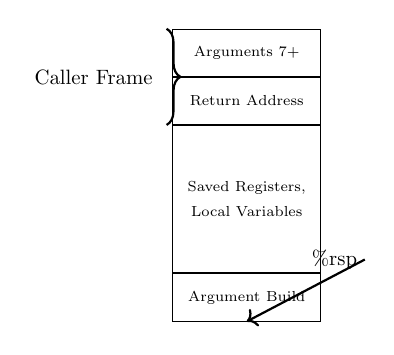
\begin{tikzpicture}[scale=0.75, transform shape]
    \node[draw, rectangle, minimum height=0.6cm, minimum width=2.5cm, minimum height=0.8cm, align=center] (args) at (0,0) {\scriptsize Arguments 7+};
    \node[draw, rectangle, minimum height=0.6cm, minimum width=2.5cm, below=0 of args, minimum height=0.8cm, align=center] (ret) {\scriptsize Return Address};
    \node[draw, rectangle, minimum height=0.6cm, minimum width=2.5cm, below=0 of ret, minimum height=2.5cm, align=center] (current) {\scriptsize Saved Registers,\\ \scriptsize Local Variables};
    \node[draw, rectangle, minimum height=0.6cm, minimum width=2.5cm, below=0 of current, minimum height=0.8cm, align=center] (build) {\scriptsize Argument Build};
    \draw[decorate, decoration={brace, amplitude=5pt}, thick] ($(args.north west)+(-0.1,0)$) -- ($(ret.south west)+(-0.1,0)$) node[midway, left, xshift=-3pt] {Caller Frame};
    \draw[thick, ->] (2, -3.5) node[left] {\%rsp} -- (build.south);
\end{tikzpicture}
\end{center}

\subsection*{Data Structures}
\subsubsection*{Arrays}
A nested array `int A[R][C]` is a single contiguous memory block. Access is `Address(A) + (i*C + j) * sizeof(int)`. A multi-level array `int* A[R]` is an array of pointers, requiring two memory accesses to get to an element.

\subsubsection*{Structures \& Alignment}
Structs group data but may include padding for alignment.
\begin{itemize}
    \item \textbf{Alignment Rule}: Data of size $K$ bytes must have an address that is a multiple of $K$.
    \item \textbf{Padding}: Compiler inserts unused bytes to align fields and ensure total struct size is a multiple of the largest field's alignment. To save space, declare larger fields first.
\end{itemize}
\begin{lstlisting}[language=c, basicstyle=\ttfamily\tiny, caption=Alignment Padding]
struct S { char c; int i; }; // sizeof is 8, not 5
// Layout: |c|pad|pad|pad|  i  |
\end{lstlisting}

\subsubsection*{Floating Point}
Uses separate **XMM registers** (\%xmm0-\%xmm15) for arguments and return values. Instructions like `addss` (single-precision) and `addsd` (double-precision) perform FP arithmetic.

\section*{Advanced Systems Concepts}

\subsection*{Linking \& Compilation}
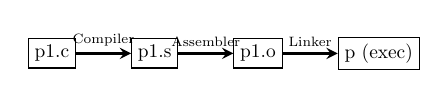
\begin{tikzpicture}[scale=0.7, transform shape]
    \node (c) [draw] {p1.c};
    \node (s) [draw, right=of c] {p1.s};
    \node (o) [draw, right=of s] {p1.o};
    \node (e) [draw, right=of o] {p (exec)};
    \draw [thick,->,>=stealth] (c) -- (s) node[midway, above, font=\scriptsize]{Compiler};
    \draw [thick,->,>=stealth] (s) -- (o) node[midway, above, font=\scriptsize]{Assembler};
    \draw [thick,->,>=stealth] (o) -- (e) node[midway, above, font=\scriptsize]{Linker};
\end{tikzpicture}
\begin{itemize}
    \item \textbf{Symbol Resolution:} Matching symbol references to definitions.
    \item \textbf{Relocation:} Updating addresses once final memory locations are known.
\end{itemize}

\subsection*{Memory and Buffers}
\begin{itemize}
    \item \textbf{Memory Layout:} Stack (grows down), Heap (grows up, `malloc`), Data (globals), Text (code).
    \item \textbf{Buffer Overflow:} Writing beyond a buffer's boundaries, a major security vulnerability.
    \begin{itemize}
        \item \textbf{Protections:} Stack Canaries, Address Space Layout Randomization (ASLR), and Non-Executable (NX) stacks help prevent attacks.
    \end{itemize}
    \item \textbf{Byte Ordering (Endianness):}
    \begin{itemize}
        \item \textbf{Little Endian (x86):} Least significant byte at lowest address.
        \item \textbf{Big Endian:} Most significant byte at lowest address.
    \end{itemize}
\end{itemize}

\subsection*{Compiler Optimization}
\begin{itemize}
    \item \textbf{Constant Folding:} Pre-calculating constant expressions.
    \item \textbf{Dead Code Elimination:} Removing unreachable code.
    \item \textbf{Common Subexpression Elimination:} Reusing results of identical calculations.
    \item \textbf{Code Motion:} Moving loop-invariant code out of loops.
    \item \textbf{Inlining:} Replacing a function call with its body.
\end{itemize}

\section*{ECF \& Memory Hierarchy}

\subsection*{Exceptional Control Flow (ECF)}
ECF is a mechanism for reacting to system events by transferring control from normal program flow to the kernel.
\begin{table}[h]
    \centering
    \caption{Types of Exceptions}
    \scriptsize
    \begin{tabular}{lll}
        \toprule
        Type & Cause & Return Behavior \\
        \midrule
        Interrupt & External event (I/O) & Returns to next instruction \\
        Trap & Intentional (syscall) & Returns to next instruction \\
        Fault & Error (page fault) & Might re-execute or abort \\
        Abort & Fatal error & Does not return \\
        \bottomrule
    \end{tabular}
\end{table}

\subsection*{Processes \& Signals}
A **process** is an instance of a running program. A **signal** is a kernel message to a process about an event.
\begin{itemize}
    \item \texttt{fork()}: Creates a near-identical child process. Returns child's PID to parent, 0 to child.
    \item \texttt{execve()}: Replaces the current process image with a new program.
    \item \texttt{waitpid()}: Parent reaps a terminated child process to prevent it from becoming a "zombie".
    \item \textbf{SIGCHLD:} Signal sent to parent when a child terminates.
    \item \textbf{SIGINT:} Sent by Ctrl-C.
    \item \textbf{SIGSEGV:} Segmentation fault (invalid memory access).
\end{itemize}

\subsection*{Memory Hierarchy}
\begin{itemize}
    \item \textbf{Locality:} The tendency for programs to access data and instructions near those they have recently accessed.
    \begin{itemize}
        \item \textbf{Temporal:} Recently referenced items are likely to be referenced again soon.
        \item \textbf{Spatial:} Items with nearby addresses tend to be referenced together in time.
    \end{itemize}
    \item \textbf{Caching:} Using smaller, faster storage (e.g., SRAM) to stage data for larger, slower storage (e.g., DRAM). Locality makes caching effective.
    \item \textbf{Cache Misses:}
    \begin{itemize}
        \item \textbf{Cold (Compulsory):} Cache is empty.
        \item \textbf{Conflict:} Multiple data objects map to the same cache block, causing evictions.
        \item \textbf{Capacity:} The working set of active blocks is larger than the cache.
    \end{itemize}
    \item \textbf{Disk Access Time} = $T_{avg\_seek} + T_{avg\_rotation} + T_{avg\_transfer}$.
\end{itemize}

\section*{Virtual Memory (VM)}
\subsection*{VM Concepts}
\begin{itemize}
    \item \textbf{Address Spaces:}
    \begin{itemize}
        \item \textbf{Virtual (VA):} Uniform address space seen by a process.
        \item \textbf{Physical (PA):} Actual addresses in hardware memory.
    \end{itemize}
    \item \textbf{Pages \& Page Tables:} VM is divided into fixed-size blocks (pages). A per-process **page table** maps virtual pages to physical pages.
    \item \textbf{Page Fault:} An exception when a referenced page is not in physical memory. The OS handles it by loading the page from disk (demand paging).
    \item \textbf{Benefits:} Efficient memory use (caching), simplified memory management, and memory protection via permission bits in Page Table Entries (PTEs).
\end{itemize}

\subsection*{Address Translation}
The Memory Management Unit (MMU) translates VAs to PAs. A **Translation Lookaside Buffer (TLB)** is a small hardware cache of PTEs to speed this up.
\begin{itemize}
    \item \textbf{VA parts:} Virtual Page Number (VPN) and Virtual Page Offset (VPO).
    \item \textbf{PA parts:} Physical Page Number (PPN) and Physical Page Offset (PPO).
    \item \textbf{Process:} VPN is used to find the PTE in the TLB or page table. The PPN from the PTE is combined with the original VPO (which is the same as the PPO) to form the physical address.
\end{itemize}
\begin{center}
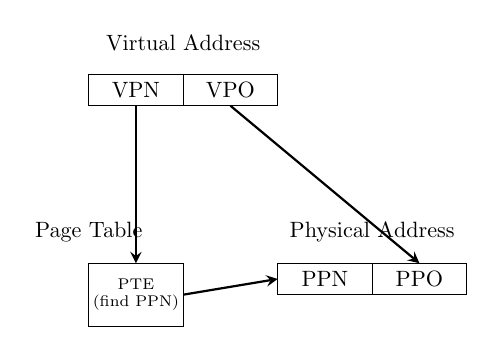
\begin{tikzpicture}[scale=0.8, transform shape]
    % Virtual Address
    \node (va_label) at (1.5, 1.5) {Virtual Address};
    \draw (0,0.5) rectangle (3,1);
    \node at (0.75, 0.75) {VPN};
    \node at (2.25, 0.75) {VPO};
    \draw (1.5,0.5) -- (1.5,1);
    
    % Page Table
    \node (pt_label) at (0, -1.5) {Page Table};
    \draw (0,-2) rectangle (1.5,-3);
    \node[align=center, font=\scriptsize] at (0.75, -2.5) {PTE \\ (find PPN)};
    
    % Physical Address
    \node (pa_label) at (4.5, -1.5) {Physical Address};
    \draw (3,-2) rectangle (6,-2.5);
    \node at (3.75, -2.25) {PPN};
    \node at (5.25, -2.25) {PPO};
    \draw (4.5,-2) -- (4.5,-2.5);

    % Arrows
    \draw[arrow] (0.75, 0.5) -- (0.75, -2);
    \draw[arrow] (2.25, 0.5) -- (5.25, -2);
    \draw[arrow] (1.5, -2.5) -- (3, -2.25);
\end{tikzpicture}
\end{center}
\begin{itemize}
    \item \textbf{Memory Mapping (`mmap`):} Creates a new VM area and associates it with an object on disk (e.g., a file or anonymous memory).
    \item \textbf{Copy-on-Write (COW):} `fork()` uses COW to defer physical memory copying until a write occurs, making process creation fast.
\end{itemize}
\end{document}